\documentclass[12pt]{article}
\usepackage[utf8]{inputenc}
\usepackage[T1]{fontenc}
\usepackage{subcaption}
\usepackage{graphicx}
\usepackage{fullpage}
\usepackage{lineno}
\usepackage[numbers,sort&compress]{natbib}
\usepackage{setspace}
\usepackage{booktabs}
\usepackage{array}
\usepackage{multirow}
\usepackage[hidelinks]{hyperref}
\usepackage{wasysym}
\usepackage{mathptmx}  % Times New Roman font
\usepackage{microtype} % improve line breaks
\DeclareMathAlphabet{\mathcal}{OMS}{cmsy}{m}{n} % Reset mathcal font to default

% \chapter{xxx}

\graphicspath {{../}}

\title{CGB: A Comparative Genomics Framework for the Analysis of
  Transcriptional Regulation in Bacteria}
\date{}

\begin{document}
\linenumbers
\doublespacing

\maketitle

\section{Introduction}

The growing number of completely sequenced genomes and increasingly available
experimentally validated transcription factor binding site (TFBS) data from
closely related species have made possible the comparative genomics analysis of
transcriptional regulatory networks in Bacteria~\cite{makarova2001conservation,
  rodionov2007comparative, babu2004structure}. In most comparative genomics
studies, however, the datasets of binding evidence and the methods used for
analysis are adopted in an ad hoc manner. The experimentally verified binding
site data usually come from a single species, or the inferred binding motifs
from multiple species are directly combined without taking into account their
phylogenetic relationship to the target genome~\cite{erill2004differences,
  novichkov2010regpredict, ravcheev2013genomic, leyn2014comparative,
  kazakov2009comparative, rodionov2008transcriptional}. Collected data is used
to transfer information from reference species to target ones using \textit{de
  facto} standard methods. Despite being reported to be effective in many
studies, these TF binding evidence transfer methods had never been evaluated in
a systematic way.

Some recent efforts to address these issues and establish standards for the
comparative genomics analyses include collecting binding site data for all
bacterial species in central repositories and systematic assessment of methods
for TF binding evidence transfer. One such effort for the data collection is
CollecTF, a database of experimentally validated transcription factor binding
sites in the Bacteria domain~\cite{kilic2013collectf}. Having binding site
evidence from an extensive collection of bacterial species, CollecTF allows
integration of TF binding evidence from a group of selected species by
dynamically aligning binding sites of possibly different lengths using
LASAGNA~\cite{lee2013lasagna}.

Although the available TF binding and regulation evidence is usually
transferred using the reference TF binding motif, there has been successful
applications of transferring transcriptional regulatory networks (TRN), rather
than the binding motif, to infer the binding motif and regulatory network in
target species~\cite{babu2008computational, novichkov2010regpredict}. We
recently evaluated transfer methods that assume conservation of the TF binding
motif (motif-based) and the methods assuming conservation of regulon
composition (network-based)~\cite{kilic2015assessment}. Our systematic
assessment showed that motif-based methods substantially outperform
network-based ones. We also found that the efficiency of motif-based transfer
methods decreases sharply with the increasing phylogenetic distance between
instances of the TF in reference and target species.

The natural step following the collection of TF binding data and applying
reliable transfer methods is the comparative analysis of predicted binding
motifs and regulons in a group of target species. Most studies use custom
implementations of computational methods to scan genomes for putative binding
sites, adopting some scoring scheme such as Position Specific Scoring Matrices
(PSSM), the Berg and von Hippel index or their
variations~\cite{schneider1986information, berg1988selection,
  osada2004comparative, beckstette2006fast}. There are also some
general-purpose platforms to analyze bacterial TF binding and regulation. One
such platform is Visual Footprint, an online framework for prediction of TF
binding sites using PRODORIC database as the data source, and for the
visualization of search results in their genomic
context~\cite{munch2005virtual, munch2003prodoric}

Another platform that allows comparative analysis of multiple genomes is
RegPredict, a system for regulon inference and comparative genomics in Bacteria
domain, integrated with the literature-based TF binding site database
RegTransBase~\cite{novichkov2010regpredict,
  kazakov2007regtransbase}. Successfully used in many comparative genomics
analysis~\cite{ravcheev2012transcriptional, antunes2012global,
  novichkov2013regprecise, galperin2014comparative}, RegPredict uses the
motif-based transfer to identify
functional sites in a group of species~\cite{kilic2015assessment}. It clusters
co-regulated orthologous operons and produces a graphical output for each
orthologous group, showing the genomic context and gene function summary
information.

Utilized in many comparative genomics analyses over the last decade, these few
existing frameworks do not meet all the demands of comparative genomics
analysis. Even though they employ motif-based transfer methods and make
accurate predictions of putative binding sites and regulated genes in each
target species, their use of ad hoc methods to combine findings in each target
genome makes hard to interpret results and test objectively the hypotheses on
transcriptional regulation of a given TF and its evolution across different
species. In addition, both Visual Footprint and RegPredict are deployed as
web-services and limit the available target genomes to those in their
collections, which makes impossible to analyze any particular genome
(complete or not fully assembled but available as multiple contigs) that is not
in the system database, which may substantially lag behind releases of the NCBI
RefSeq database.

It is useful that the TFBS data from PRODORIC and RegTransBase are directly
accessible from these platforms. However, there is no way to combine evidence
from multiple sources except simply concatenating motifs or using manually
curated ones. More importantly, the fact that both frameworks use PSSM scores
to report sites on promoter regions forces the user to predefine a PSSM score
threshold and makes the confidence level of each prediction unclear. Finally,
results for a group of orthologous operons do not exploit the phylogenetic
information and the reconstruction of the regulation state in ancestral clades,
essential elements to test the hypotheses on the evolution of transcriptional
regulation of operons. Furthermore, the combinatorial nature of operon
evolution results in multiple disaggregated results that make it hard to assess
the evolution of regulation of individual gene components. Since the gene, and
not the operon, is the essential unit under selection for regulation, the use
of an operon-based framework for its study appears misguided.

To address the shortcomings of existing comparative genomics frameworks, and to
leverage recent efforts on the availability of experimental data and the
evaluation of transfer methods, we have developed CGB, a comparative genomics
platform to analyze the transcriptional regulation in bacterial clades, using
the TF-binding evidence from one or more reference species. CGB allows the
analysis of any target genome in the NCBI RefSeq
database~\cite{o2015reference}, available as a complete genome or a set of
contigs. It incorporates the binding evidence from each reference species using
a weighted approach taking into account the phylogenetic distances and the size
of each binding site collection. Another significant contribution is the
adoption of a Bayesian framework, originally introduced for the analysis of
transcriptional regulatory networks in metagenomic
data~\cite{hobbs2016bayesian}. The use of a Bayesian framework allows
calculation of posterior probability of regulation for each operon, rather than
just reporting PSSM scores higher than a predefined threshold. The Bayesian
framework also allows incorporating prior belief on the TF-regulation of any
gene. Reporting posterior regulation probabilities for each gene yields more
interpretable and compact results than reporting raw PSSM scores on operons. Finally,
CGB performs real-time detection of orthologous genes across target genomes and
ancestral state
reconstruction for each orthologous groups of genes, enabling reliable testing
of hypotheses on the evolution of transcription factors, their binding motifs
and regulatory networks across different
organisms~\cite{pagel1999inferring}. CGB is available under a GPL license
on GitHub (\url{http://www.github.com/erilllab/cgb}).

\section{Regulation Inference and Comparative Analysis Pipeline}

The regulon inference procedure starts with the automatic download and parsing
of records for reference TF-instances and target genomes from NCBI Protein and
RefSeq databases, respectively (Figure~\ref{fig:pipeline}). The next step is
the identification of TF-instances in all target species and the reconstruction
of an approximate phylogeny of the species under analysis using the protein
sequences of all detected TF-instances. Then, for each target genome, all TFBS
collections are combined into a TF-binding model specific for each species
under analysis. Enabling the phylogenetic weighting option allows building
different TF binding models (i.e. PSSMs) for each target genome where the
contribution of each reference collection is weighted by the phylogenetic
distance between its source and the target genome.

\begin{figure}
  \centering
  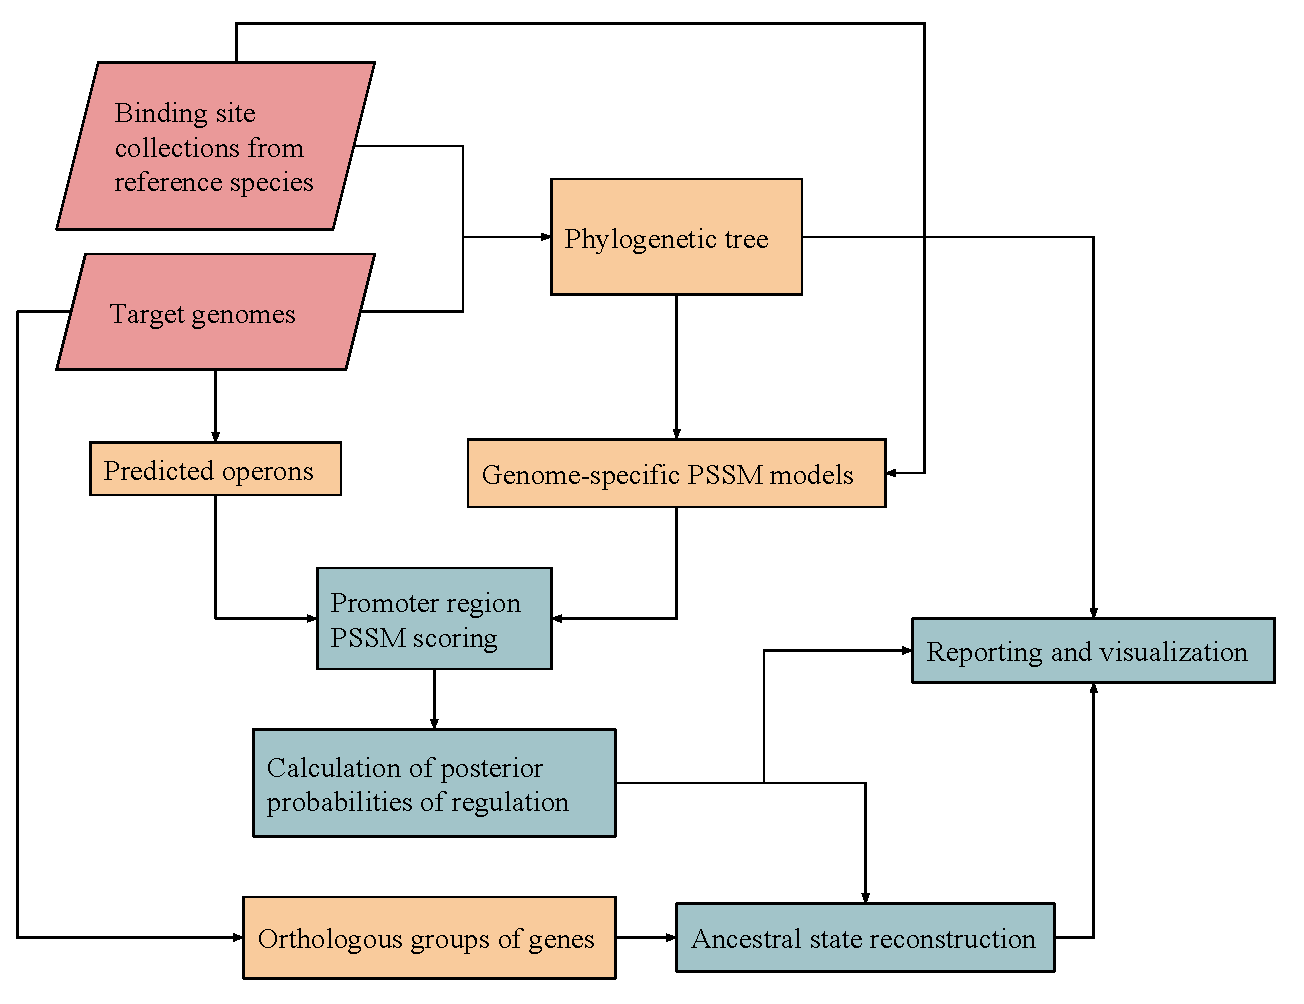
\includegraphics[width=\textwidth]{figures/chapter4/cgb_workflow}
  \caption{The comparative genomics workflow implemented in CGB\@. Input TFBS
    collections from reference species are combined to build a PSSM model for
    each target species where the the site collection from each reference
    species is weighted by its phylogenetic distance to the target
    species. Upstream regions of predicted operons are PSSM-scored and
    posterior probability of regulation for each operon is calculated. For each
    orthologous group of genes, the likelihood of gene regulation in common
    ancestors are inferred through ancestral state reconstruction.}
  \label{fig:pipeline}
\end{figure}

The next step, for each target genome, is to predict operons and score their
upstream regions for putative binding sites. Given a promoter region scored by
its genome-specific PSSM, all scores are combined into a posterior probability
of TF binding to the promoter region, under the assumption that TF-binding is
functionally linked to the regulation of the downstream operon. Once all the
operons have their regulation probabilities computed, operon genes are assigned
via reciprocal BLAST to orthologous groups, where each group contains at most
one gene from each target genome and each gene is orthologous to other genes in
the same group.

The final step of the pipeline is ancestral state reconstruction. Given the
phylogeny and an orthologous group of genes,  ancestral reconstruction is
performed to infer the state of TF regulation in ancestral clades.

As output, the putative binding sites in promoter regions of all target genomes
are reported in Comma-Separated Value (CSV) format. Also, the phylogenetic tree
that is built with TF-instances from reference and target species is produced
in Newick and Nexus formats~\cite{maddison1997nexus,
  felsenstein2004inferring}. In addition to genome-specific reporting of all
operons and their posterior probabilities of regulation, the orthologous groups
of genes and their regulation probabilities are reported together to compare
the TF-regulation of the same gene in different organisms. These results are
visualized as a heatmap (Figure~\ref{fig:heatmap_2}), presented with the
phylogenetic tree, where each row corresponds to an orthologous group, and each
column denotes the genes of a single genome~\cite{huerta2016ete}. Each gene is
represented as a square in the heatmap and its color is based on the posterior
probability of its regulation, ranging from green (probability of one) to red
(probability of zero). The absence of an ortholog in a species for a particular
ortholog group is indicated in blue color. Finally, for each gene, the
TF-regulation probabilities in each target species and in their shared ancestors are
visualized with the phylogenetic tree.

The following subsections describe each step of the workflow in detail.

\subsection{TF binding evidence and genome processing}

The TF binding evidence from each organism is defined as the collection of
binding sites and the NCBI protein accession numbers of the TF-instance. The
target genomes are defined as the pair of user-defined strain names and NCBI
RefSeq accession numbers of each chromosome, plasmid or contig of the
species. The protein and genome records are downloaded via Entrez queries, and
the genome annotations are parsed using Biopython~\cite{wheeler2007database,
  cock2009biopython}. The TF-instances on target genomes are identified via
BLAST (tblastn) using reference TF-instances as query
sequences~\cite{altschul1990basic}. If there are multiple reference
TF-instances and they have best BLAST hits to different genes of a target
genome, the BLAST hit with the smallest e-value is selected. The target genomes
with no identified TF-instance are discarded from the analysis.

\subsection{Operon prediction}

The distance between two adjacent genes is a powerful indicator whether genes
are in the same operon~\cite{westover2005operon}. Genes that are in the same
operon tend to be closer to each other than adjacent genes in different
operons. CGB predicts operons of a given genome using a distance threshold,
such that all directon gene pairs (adjacent genes on the same DNA strand with
no intervening gene on the other strand) with intergenic distance less than the
threshold are considered to belong to the same operon~\cite{salgado2000operons,
  moreno2002powerful, price2005novel}. Since CGB does not restrict the target
genomes to a limited set, it is not feasible to rely on existing operon
databases which contain operon predictions for a fixed set of
genomes~\cite{mao2009door, taboada2012proopdb, pertea2009operondb}. Other
operon prediction methods based on conserved features, functional similarity
and codon usage are not suitable either, since using them would require having
many closely related genomes to calculate comparative features for any target
genome, dramatically increasing runtime~\cite{chuang2012features}. There exist
operon prediction methods that rely on the identification of sequence motifs
pertaining to promoter and terminator sites, but these methods are known to be
of limited applicability, since these sequence elements are not well conserved
across bacterial species~\cite{salgado2000operons, itoh1999evolutionary}. To
address these limitations, CGB relies on the use of an intergenic distance
threshold to predict operons. Although known to overestimate the number of
operons (by splitting real operons), this method is known to have relatively
high accuracy as operon predictor and has been widely
used in the literature~\cite{chuang2012features, westover2005operon}. A main
limitation of intergenic distance-based methods stems from the fact that
different genomes may display lower or higher compaction in their intergenic
regions. Rather than using a single
threshold for all target genomes, CGB uses a specific threshold for each target
genome, which is determined based on its intergenic distance distribution.

In order to determine the optimal method to automatically define an intergenic
distance threshold on each target species, we performed a benchmark of several
alternative methods using available data on operon organization across the
Bacteria domain. Pperons of species with more than 500 known operons were
retrieved from ODB operon database~\cite{okuda2006odb}. Each adjacent gene pair
was labeled as a WO (within-operon) pair or a TUB (transcription unit boundary)
pair~\cite{chen2004computational}. Species with known operons available in ODB
are \textit{Bacillus subtilis} subsp. subtilis 168 (bsu), \textit{Escherichia
  coli} K-12 MG1655 (eco), \textit{Helicobacter pylori} 26695 (hpy),
\textit{Listeria monocytogenes} EGD-e (lmo), \textit{Corynebacterium
  glutamicum} ATCC 13032 (cgb) and \textit{Legionella pneumophila} Paris (lpp).

Figure~\ref{fig:operon-prediction-a} shows that using a single intergenic
distance threshold for all species would not perform well since intergenic
distances within operons vary across
species~\cite{rogozin2002congruent}. Therefore, for a given genome, the
distance threshold can be calculated using the intergenic distance distribution
of adjacent genes on the same strand. Given that about half of all protein
coding genes in bacterial genomes are located in operons~\cite{price2006life} and pairs
of adjacent genes within the same operon tend to be closer than pairs of genes
in different operons, Figure~\ref{fig:operon-prediction-b} demonstrates that
mean intergenic distance of adjacent genes on the same strand is a good
estimator of the optimal intergenic distance threshold.

\begin{figure}
  \centering
  \begin{subfigure}{\textwidth}
    \centering
    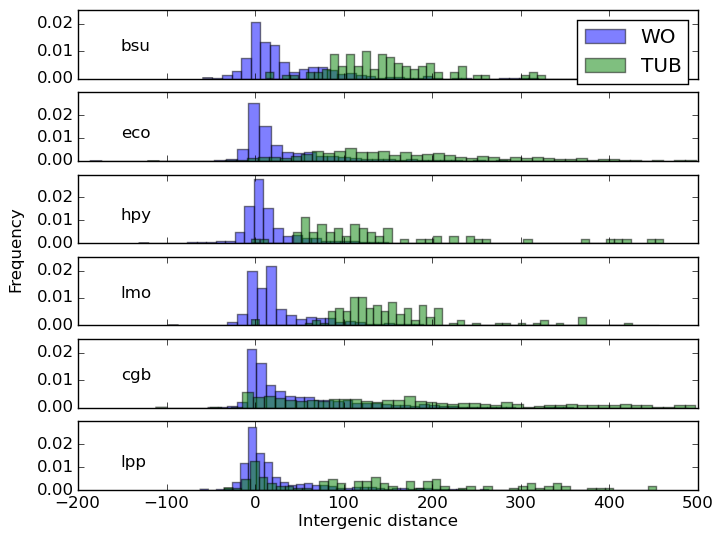
\includegraphics[width=0.6\textwidth]{figures/chapter4/operon_prediction_1}
    \subcaption{Histograms of intergenic distances of adjacent genes that are
      on the same strand. They demonstrate that pairs of genes within the same
      operon (WO) are closer than pairs in different operons (TUB). Also, the
      intergenic distance distribution is different for each species.}
    \label{fig:operon-prediction-a}
  \end{subfigure}

  \begin{subfigure}{\textwidth}
    \centering
    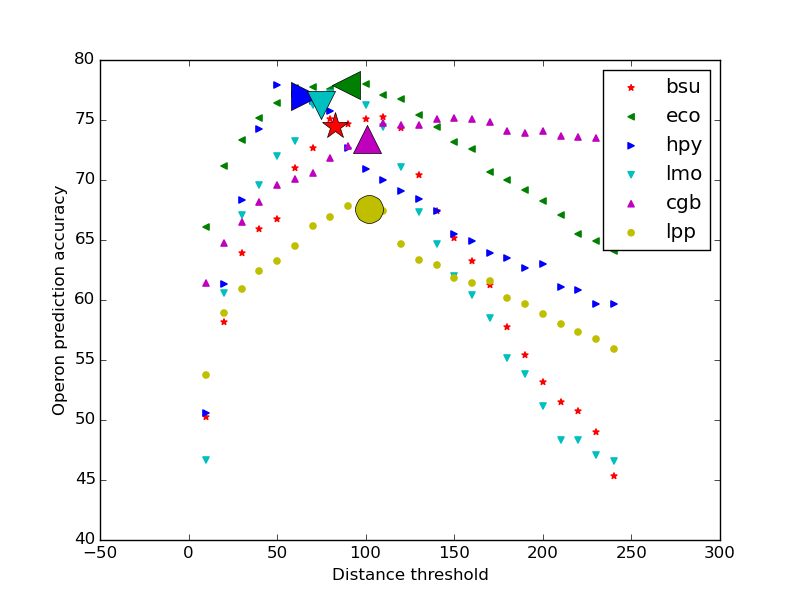
\includegraphics[width=0.6\textwidth]{figures/chapter4/operon_prediction_2}
    \subcaption{Percent operon prediction accuracy as a function of intergenic
      distance threshold (bp). The mean intergenic distances and the prediction
      accuracy of using them as thresholds are shown with larger markers. Since
      operons are predicted to search for binding sites, each operon is
      evaluated as a structure of regulation. Hence, accuracy is defined as the
      ratio of genes that are assigned to their true promoter.}
    \label{fig:operon-prediction-b}
  \end{subfigure}

  \caption{Determining the species-specific intergenic distance threshold for
    operon prediction.}
  \label{fig:operon-prediction}
\end{figure}

Following the first pass based on intergenic distance threshold, operon
predictions are enhanced using information of putative binding sites identified
on the genome-wide search process. Given that functional binding sites are very
unlikely to occur anywhere except in promoter regions, the upstream regions of
all genes, intra- and inter-operon, are searched for putative binding sites and
all operons that contain a high-scoring putative site upstream of an internal
gene (i.e.\ any gene of the operon except the first one) are split into two
operons at the point where the putative binding site lies. It should be noted
that the PSSM score threshold that determines what is considered a high-scoring
TF-binding site is used only to improve operon prediction, not to identify
binding sites to infer regulation. The selected PSSM score threshold satisfies
the equality between the negative logarithm of the false positive rate (FPR)
and the information content (IC) of the motif~\cite{hertz1999identifying}.

\subsection{Phylogenetic weighting of binding evidence}

The phylogenetic tree, used to weight binding evidence from reference species
and to perform ancestral state reconstruction, is reconstructed using the
pairwise protein sequence alignments of TF-instances of the reference and target
genomes. The midpoint rooted tree is generated using the neighbor-joining
method and pairwise distances are calculated as percentage identities of the
alignments~\cite{saitou1987neighbor}.

The TFBS collections from all reference species are combined into a distinct
binding model for each target species. For a given target genome, the
contribution of each reference collection is weighted proportional to its size
and inversely proportional to the phylogenetic distance between reference and
target species. The rationale for weighting the evidence by site count is that
the collections with more binding sites are more likely to be complete
collections; therefore, they tend to be more useful to infer putative sites in
target genome. The motivation for weighting the binding site collections by
their phylogenetic distances to the target genome is that the collection from a
closely-related species is more likely to have a similar binding motif than
that of a more distantly related species. To avoid that the inferred TF binding
model in a target species be dominated by the evidence from many closely
related-species, the contribution of each referenced collection is adjusted
using the phylogeny, following the method that CLUSTALW uses to weigh sequence
contributions for multiple sequence
alignment~\cite{thompson1994clustal}. Multiple sources of evidence originating
from a shared branch of the tree are down-weighted according to the number of
sources in that subtree. Conversely, solitary sources of evidence in a subtree
are up-weighted to equalize their contribution with that of more populated
areas of the tree.


\subsection{Bayesian estimation of regulation probabilities}

Given multiple TF binding site collections that the TF binds in different
species, we combine their PSFMs using a weighted average and transform the
combined PSFM into a PSSM assuming uniform background distribution. For each
operon, we score both strands of a predefined promoter region [300 bp upstream
to 50 bp downstream with respect to transcriptional start site by default]. For
each sequence position, we combine the scores from both strands using the
softmax function:

\begin{equation}
  PSSM(s_i) = \log_2 (2^{PSSM(s_i^f)} + 2^{PSSM(s_i^r)})
\end{equation}
where $PSSM(s_i )$ is the PSSM score of the site starting at position $i$ and
$PSSM(s_i^f)$ and $PSSM(s_i^r)$ are the scores of the site at position $i$ in
forward and reverse strands, respectively~\cite{hobbs2016bayesian}.

To estimate the probability of regulation for each operon, we define two
distributions for the set of PSSM scores of promoter regions. If the TF does
not regulate a given operon, we expect that the PSSM scores of its promoter
region follow a background distribution of scores $B$ which we approximate by a
normal distribution parameterized by the statistics of all promoters in the
genome.

\begin{equation}
  B \sim N(\mu_g, \sigma_g^2)
\end{equation}

On the other hand, for the operons regulated by the TF, the distribution of
PSSM scores should be a mixture of the background distribution and the
distribution of scores in functional sites.

\begin{equation}
R \sim \alpha N(\mu_m, \sigma_m^2) + (1-\alpha) N(\mu_g, \sigma_g^2)
\end{equation}

To quantify how likely a gene is to be regulated by the TF, instead of relying
on TF binding scores, we employ a Bayesian framework to calculate posterior
probabilities of binding which has a natural
interpretation~\cite{hobbs2016bayesian}. We define the probability of
regulation of an operon as the posterior probability of the mixture
distribution of scores ($R$), given the PSSM scores of its promoter region
($D$):

\begin{equation}
P(R|D) = \frac{P(D|R)P(R)}{P(D)} = \frac{P(D|R)P(R)}{P(D|R)P(R) + P(D|B)P(B)}
\end{equation}

The likelihood functions $P(D|R)$ and $P(D|B)$ can be defined for a given score
$s_i$ using the density functions described above ($R$ and $B$). Assuming
independence among the scores at different positions, the likelihood functions
are defined as

\begin{equation}
  P(D|R) = \prod_{s_i \in D} \mathcal{L}(s_i|R) =
  \prod_{s_i \in D} \mathcal{L}(s_i | \alpha N(\mu_m, \sigma_m^2) + (1-\alpha)N(\mu_g,\sigma_g^2))
\end{equation}
and

\begin{equation}
  P(D|B) = \prod_{s_i \in D} \mathcal{L}(s_i|B) = \prod_{s_i \in D} \mathcal{L}(s_i | N(\mu_g, \sigma_g^2))
\end{equation}

The computation of the Bayesian posterior probability $P(R|D)$ requires that
the priors $P(R)$ and $P(B)$ be defined. In addition to the option of manually
setting the prior $P(R)$, we provide two alternatives that can be used
depending on the reference collections. First, assuming that the reference
binding collections are nearly complete, the prior probability of regulation
$P(R)$ can be inferred directly based on the sizes of reference collections,
dividing the known number of regulated operons by the total number of operons
predicted in the genome. Using the weights assigned to each reference
collection, we define for each species $P(R)$ as the weighted average of site counts on each
reference TF binding motif:

\begin{equation}
P(R) = \sum_i w_i \frac{|M_i|}{|\mathcal{O}_i|}
\end{equation}
where $w_i$ is the weight associated with the reference motif $M_i$, $|M_i|$ is
the size of the $i$th collection and $|\mathcal{O}_i|$ is the number of
predicted operons of its genome. The second method is based on the
informational requirements on TF binding motifs~\cite{schneider1986information,
  schneider2000evolution, o2014informational}. Given the approximate equality
$R_{\mathrm{sequence}} \approx R_{\mathrm{frequency}}$, the expected number of
functional binding sites is $|\mathcal{G}| / 2^{R_{\mathrm{sequence}}}$ where
$|\mathcal{G}|$ is the genome sequence length. Expecting one binding site per
regulated operon, we define the prior probability of regulation $P(R)$ as

\begin{equation}
P(R) = \frac{|\mathcal{G}|}{2^{R_{\mathrm{sequence}}} |\mathcal{O}|}
\end{equation}

\subsection{Ortholog detection and ancestral state reconstruction}

For the comparative analysis of TF regulation, we identify orthologous groups
of genes using the best reciprocal BLAST hit
approach~\cite{wall2003detecting}. Given the phylogenetic tree and the inferred
posterior probabilities of regulation for genes in an orthologous group, we
infer the state of regulation of the gene in ancestral species using ancestral
state reconstruction. We use BayesTraits, a trait evolution analysis tool, to
perform ancestral reconstruction of discrete states by fitting a
continuous-time Markov model~\cite{pagel2004bayesian}. The rates of transitions
among discrete states are estimated based on the distribution of states among
the species. Given the estimated state transition rates, the ancestral states
are reconstructed by calculating the likelihood of observing the states of
species, having fixed the ancestral node at all possible states. The state of
the ancestral node is determined as the one that maximizes the likelihood of
observing the species data~\cite{pagel1997inferring, pagel1999maximum}.

For each orthologous group, we determine the discrete states of each species
based on their inferred posterior probabilities of regulation. That is, for
each species that have a gene in the orthologous group, the state takes the
value $s_1$, the state of regulation, with probability of $P(R|D)$ and the
value $s_0$, the state of not regulation, with probability of
$P(B|D)=1-P(R|D)$. For species that do not have any gene in the orthologous
group, the state is set to $s_A$, the state of absence of the gene. Repeating
the discretization process 1,000 times and estimating the discrete states on
ancestral nodes of the phylogenetic tree, we combine the results of each
iteration back into probabilities, $P(s_1)$, $P(s_0)$ and $P(s_A)$, by counting
the frequency of each state in 1,000 iterations (Figure~\ref{fig:asr}).

\begin{figure}
  \centering
  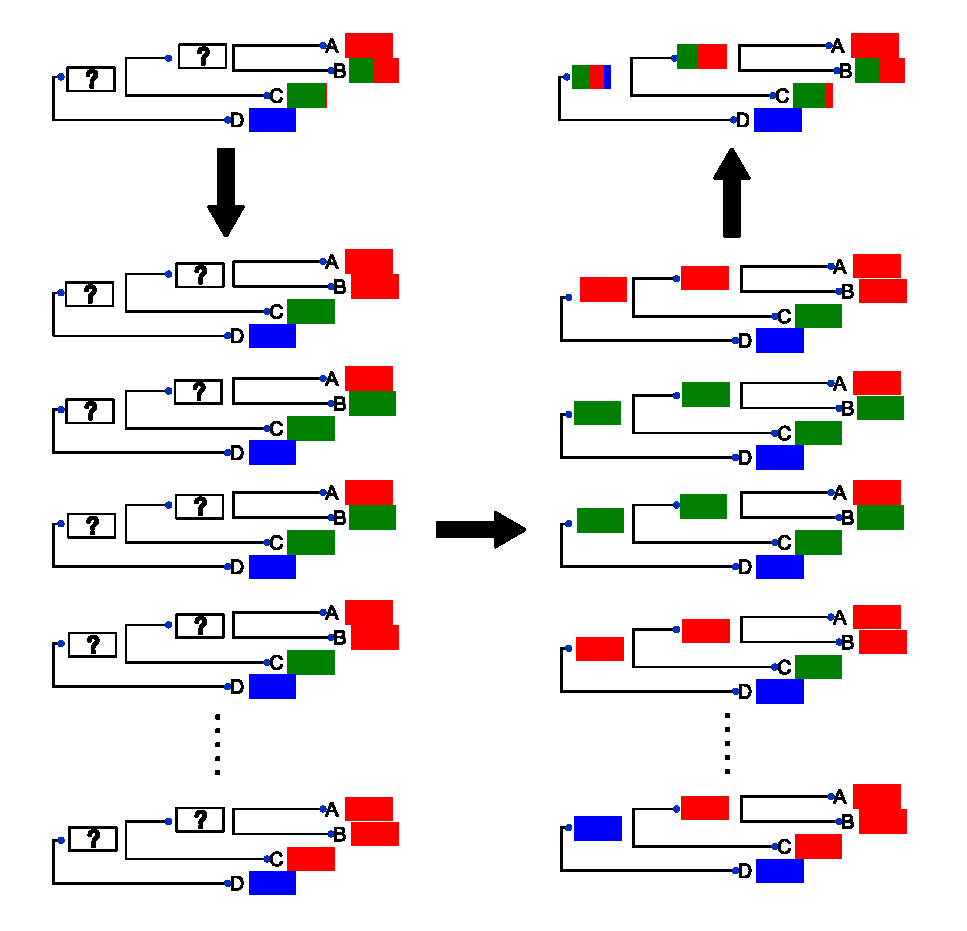
\includegraphics[width=0.8\textwidth]{figures/chapter4/asr}
  \caption{Ancestral state reconstruction for a group of orthologous genes.
    First, for each target species, the probabilities of each state is set
    based on posterior probability of gene regulation. If a given species has
    the copy of the gene, $P(s_1) = P(R|D)$, $P(s_0) = 1-P(R|D)$ and
    $P(s_A) = 0$.  Otherwise, $P(s_A) = 1$ and $P(s_1) = P(s_0) = 0$. For the
    ortholog in each species, the state is discretized 1,000 independent times
    according its associated probabilities. The states in common ancestors are
    inferred in all 1,000 trees with discrete states through ancestral state
    reconstruction. The state probabilities, $P(s_1)$, $P(s_0)$ and $P(s_A)$ on
    each internal node of the tree are defined as relative frequencies of the
    states $s_1$, $s_0$ and $s_A$, respectively, in the resulting 1,000 trees
    on which discrete ancestral state reconstruction has been performed.}
  \label{fig:asr}
\end{figure}

\subsection{Command-line and graphical interface}

CGB is publicly available with both command-line and graphical
interfaces. In command-line interface, the user provides the input, the binding
site collections, target genome accession numbers and configuration parameters,
as a text file in JSON format~\cite{bray2014javascript} and the results are
saved to files in the working directory. When using the graphical
interface, the user provides the input through a form and browses the results
rendered as HTML tables where the user can sort by posterior probabilities or
genomic position, and search the results table for gene names, locus tags or product
functions (Figure~\ref{fig:gui-input} and~\ref{fig:gui-output}).

\begin{figure}
  \centering

  \begin{subfigure}{\textwidth}
    \centering
    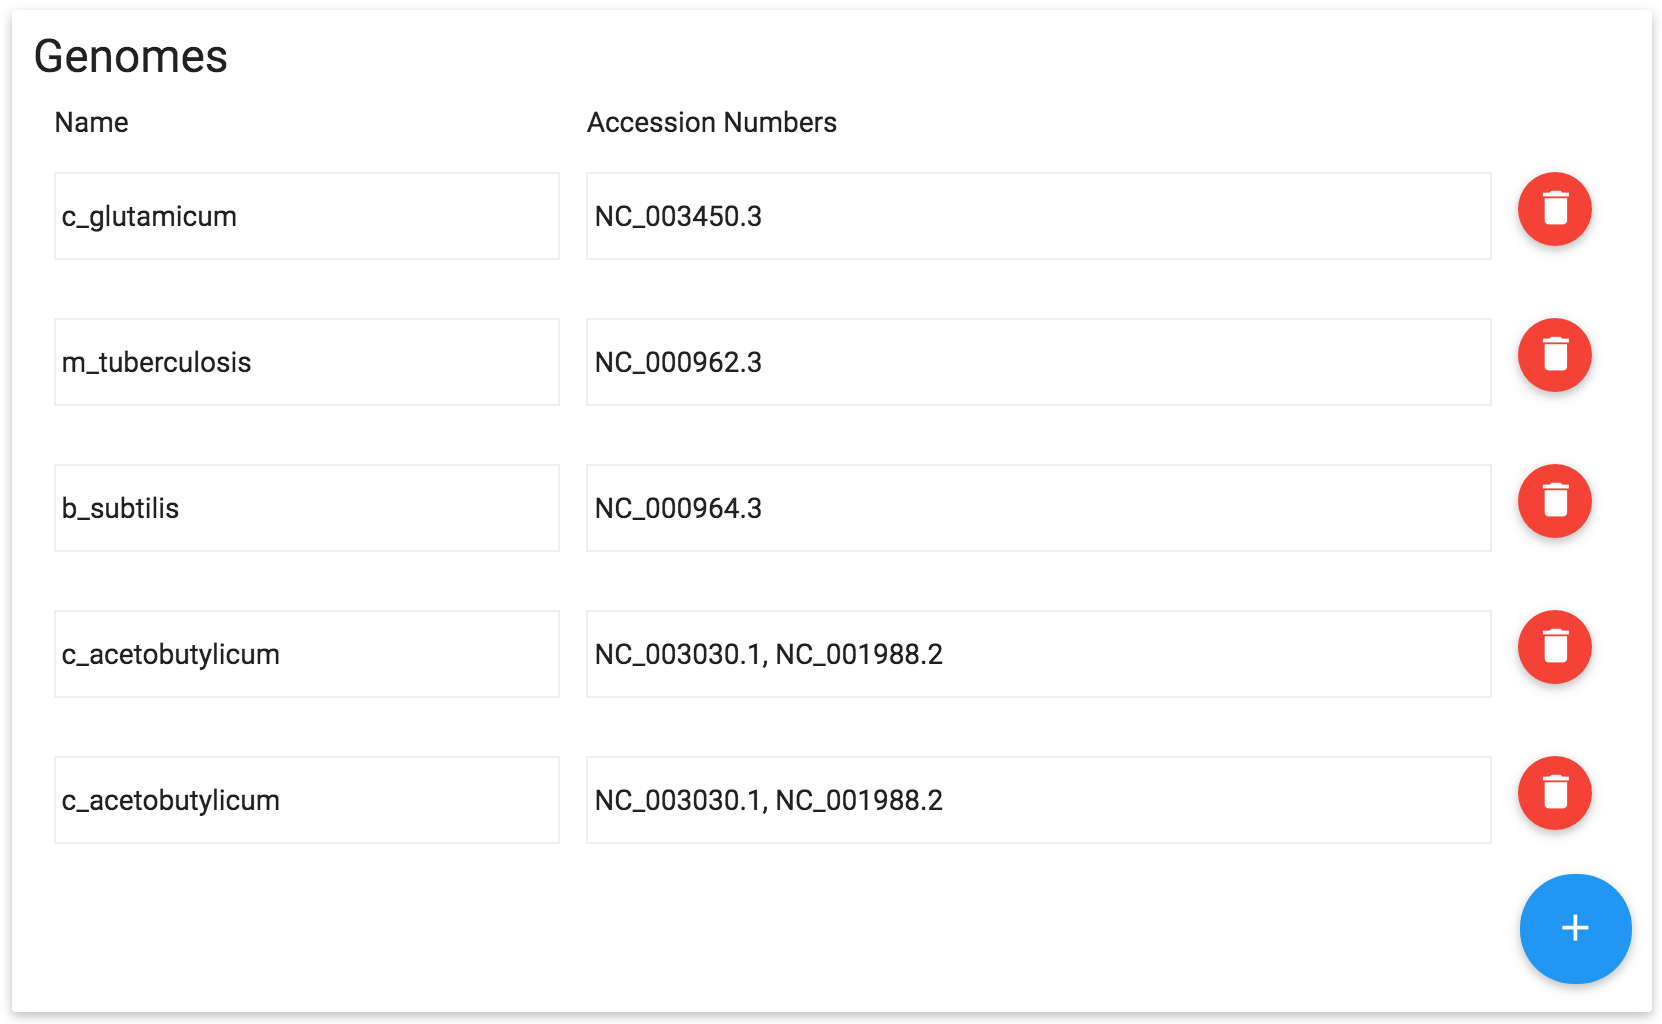
\includegraphics[width=0.6\textwidth]{figures/chapter4/input_genomes}
  \end{subfigure}

  \begin{subfigure}{\textwidth}
    \centering
    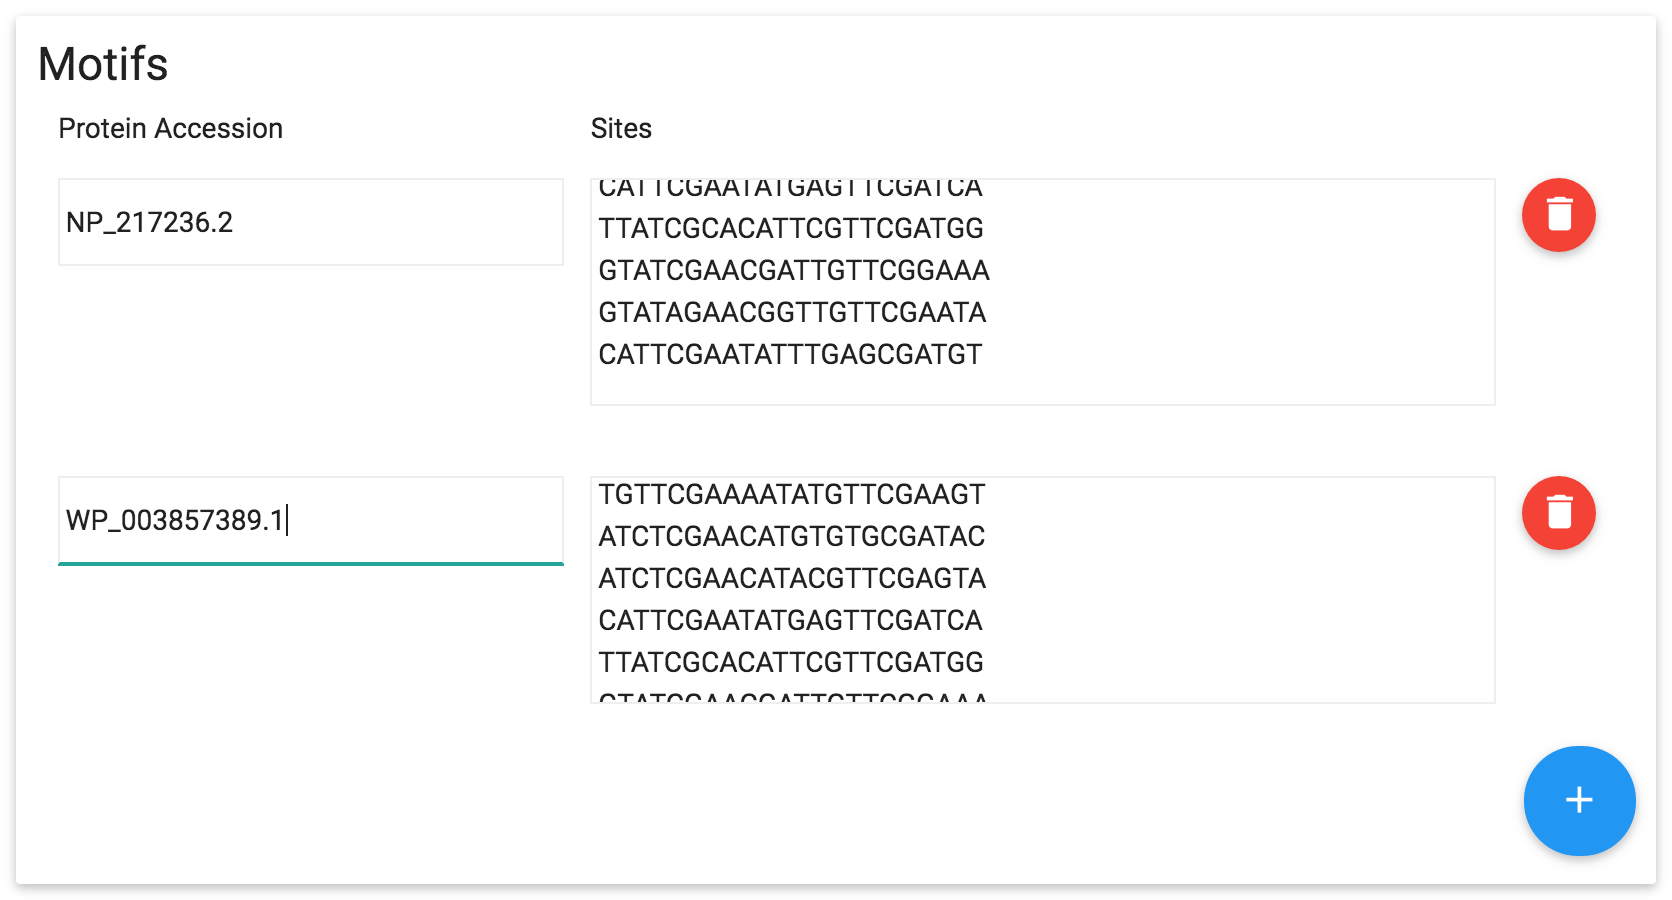
\includegraphics[width=0.6\textwidth]{figures/chapter4/input_motifs}
  \end{subfigure}

  \begin{subfigure}{\textwidth}
    \centering
    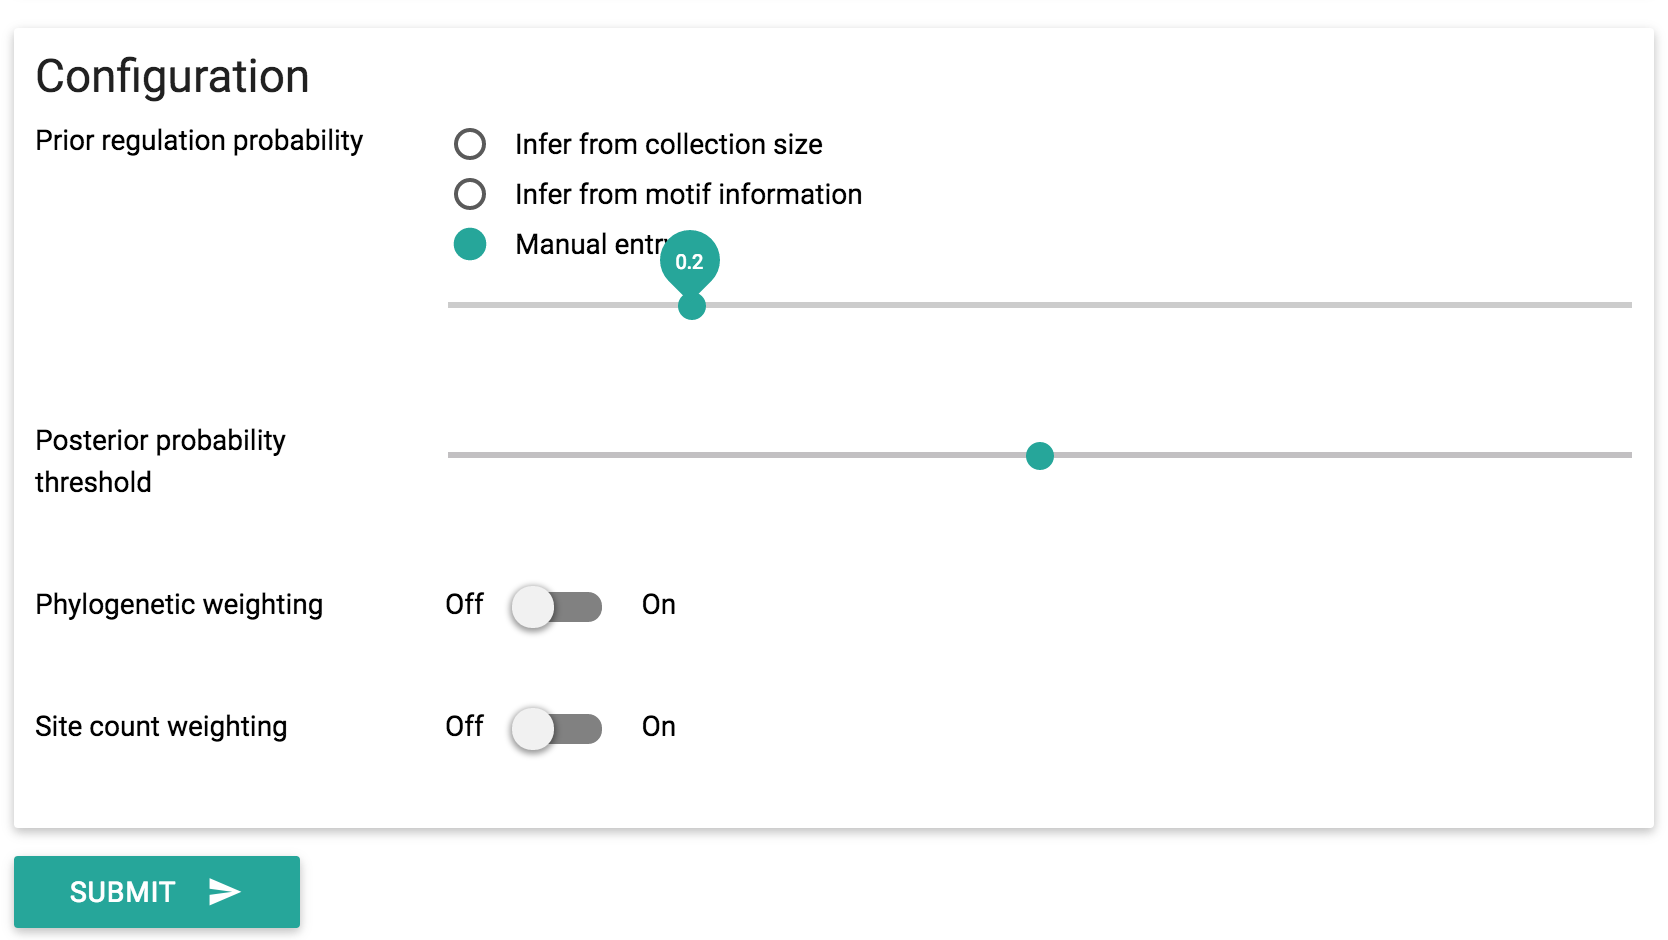
\includegraphics[width=0.6\textwidth]{figures/chapter4/input_config}
  \end{subfigure}
  \caption{The input form contains the list of genomes under analysis,
    reference TFBS collections and configuration parameters. For each target
    genome, a user-defined name and accession numbers for its all chromosomes,
    plasmids or contigs are entered. For each reference collection of binding
    sites, the accession number of the protein and the list of sites are
    entered. Finally, the configuration parameters, the method for calculating
    the prior probability (inferring from collection sizes, combined binding
    motif or manual entry), and whether binding motifs should be weighted by
    site counts and phylogenetic proximity are set.}
  \label{fig:gui-input}
\end{figure}

\begin{figure}
  \centering
  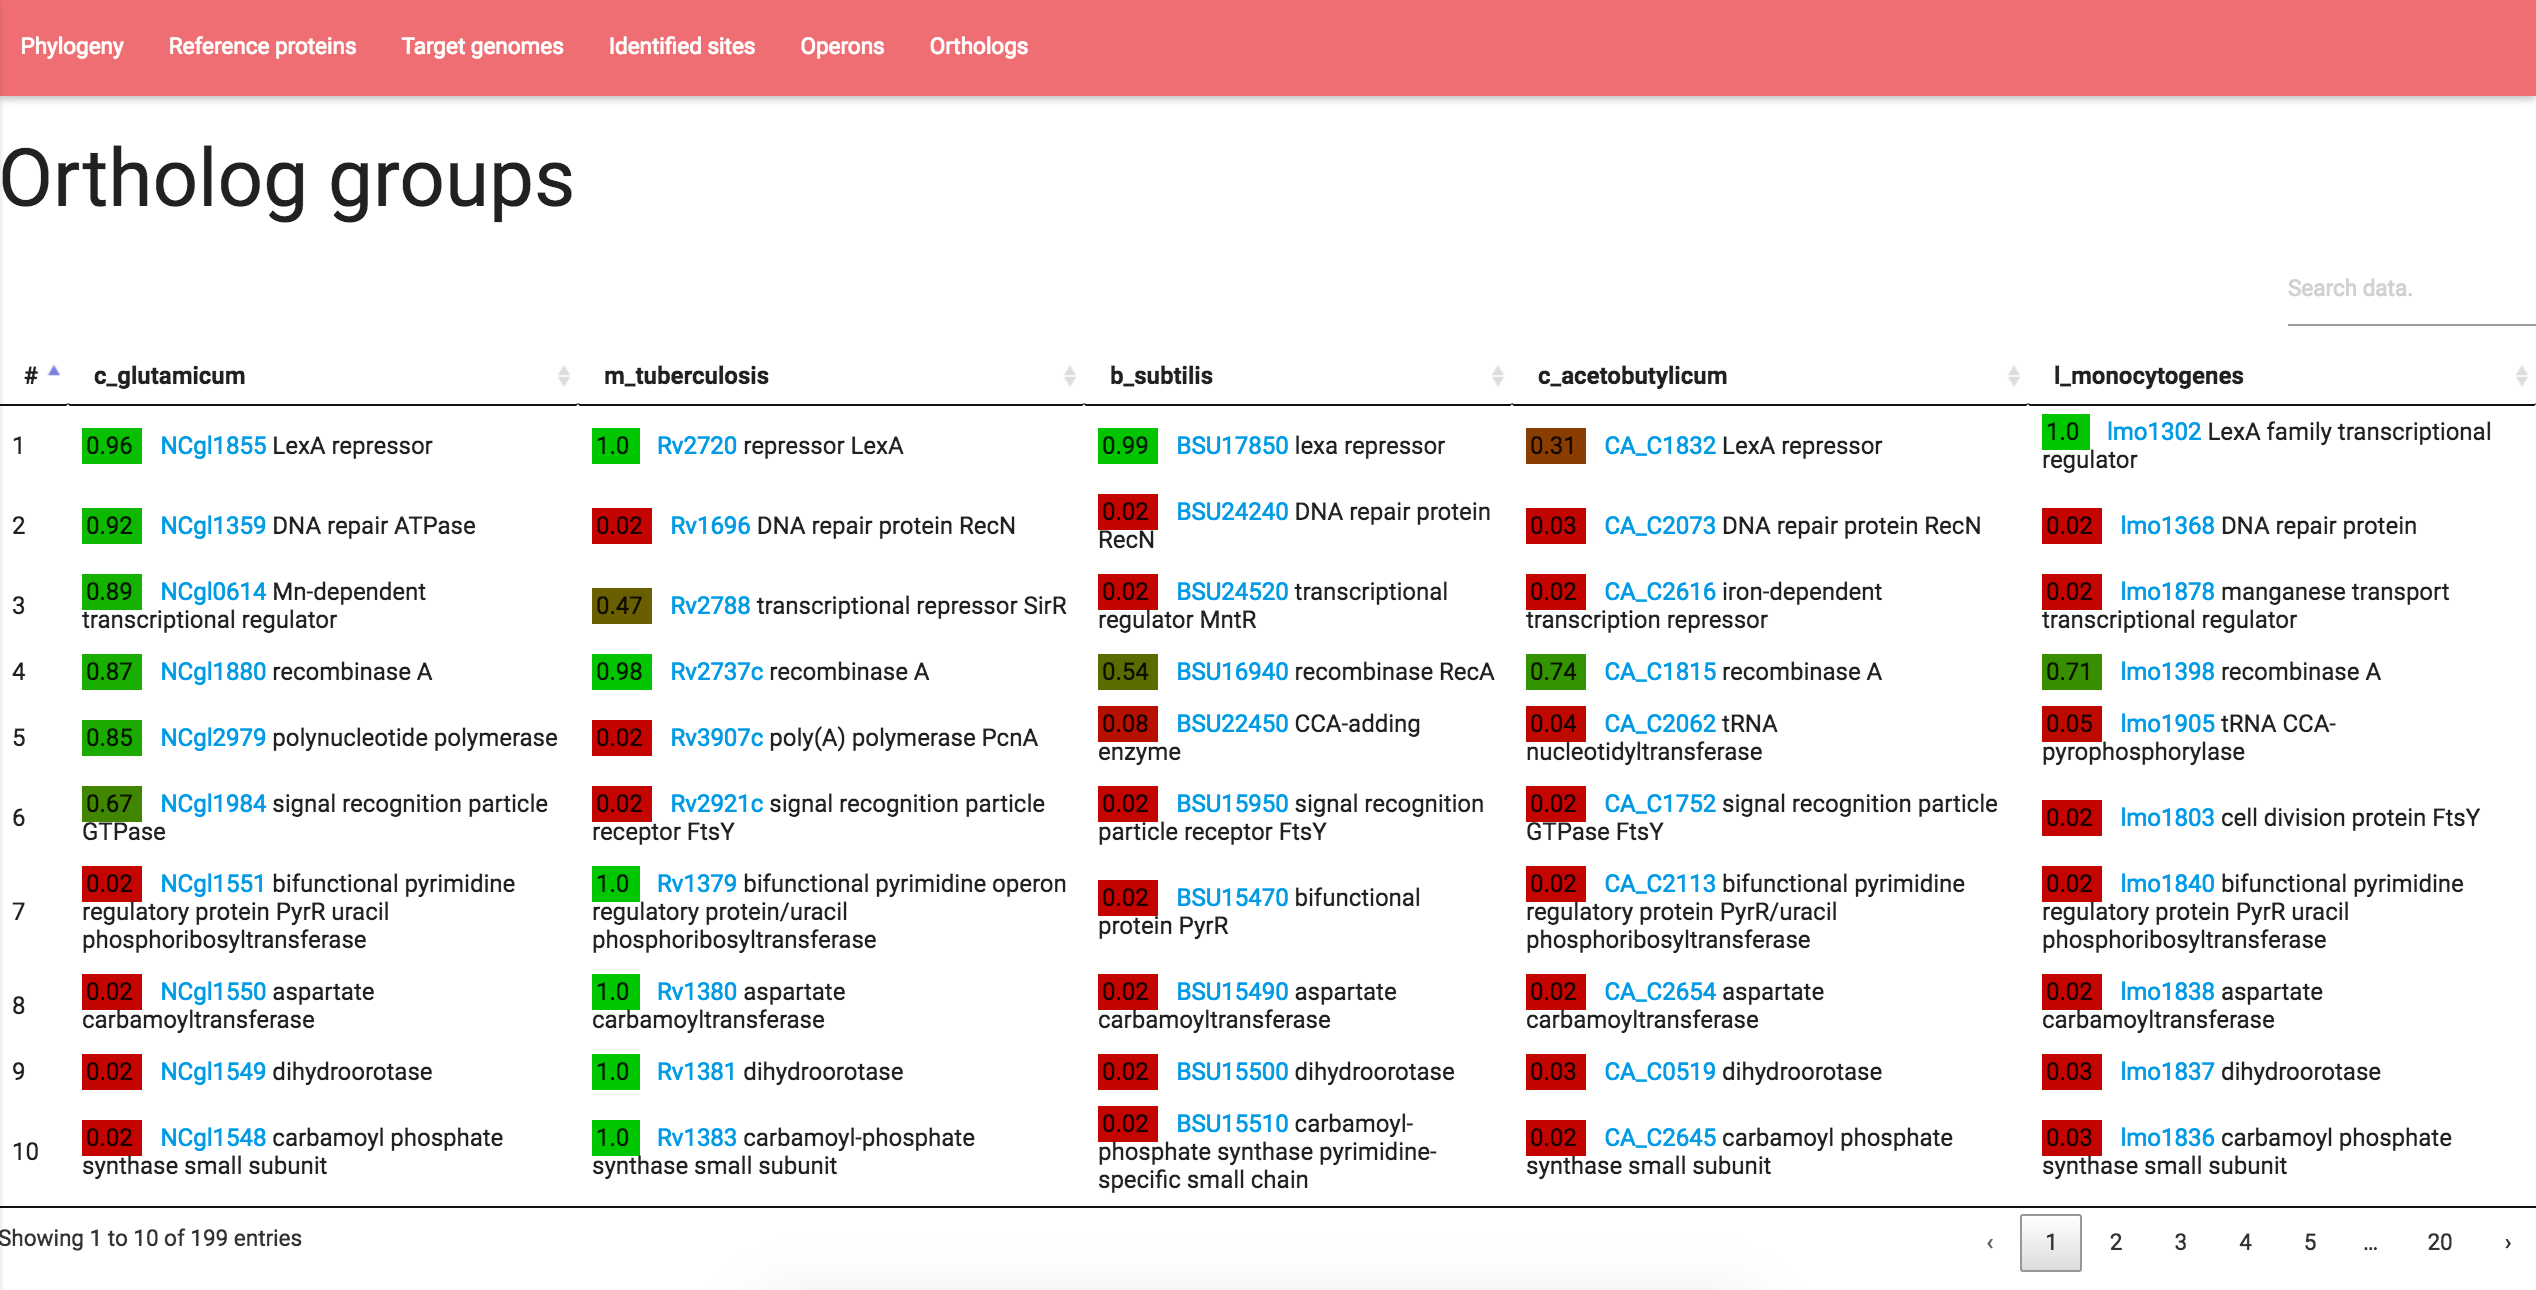
\includegraphics[width=\textwidth]{figures/chapter4/output}
  \caption{Table of ortholog groups as a part of CGB graphical interface
    output. Each row showing a group of orthologous genes from each species,
    their functions and calculated posterior probabilities of regulation. The
    table can be sorted and searched by the gene name, locus tag, function or
    probability values. In addition, the phylogeny of the species under
    analysis, the list of predicted operons and binding sites in each species
    are displayed as tables. The heatmap and reconstructed ancestral
    TF-regulation state visualizations are also available in the graphical
    interface. All results can be exported for further analysis.}
  \label{fig:gui-output}
\end{figure}

\section{Comparative genomics of LexA regulation in Gram-positive Bacteria}

The primary mechanism for controlling the response to DNA damage in Bacteria is
the SOS response, regulated by the transcription factor
LexA~\cite{radman1975sos, erill2007aeons, michel2005after}. During normal
growth, LexA binds as a homodimer to specific sites upstream of genes and
blocks their regulation. When DNA damage occurs, single-stranded DNA
accumulates originating at replication forks. The other key protein in the
mechanism, RecA forms filaments around the single-stranded DNA fragments and,
thereby promotes LexA self-cleavage which induces the SOS response.

Unlike many other transcriptional regulators, LexA has binding motifs that vary
significantly across different phyla. It has been reported that LexA binds to
short inverted repeats (\texttt{GAAC-N4-GTTC}) in the Firmicutes and
Actinobacteria~\cite{au2005genetic, davis2002definition}, whereas it displays
larger palindromic motifs (\texttt{CTGT-N8-ACAG}) in the
Gammaproteobacteria~\cite{erill2003silico,
  fernandez2000identification}. Moreover, its binding motif is in the form of
direct repeat (\texttt{GTTC-N7-GTTC}) in the
Alphaproteobacteria~\cite{erill2004differences, fernandez1998identification}.
This variability makes LexA an ideal example for the study of the evolution
of transcriptional regulatory networks.


In this section, we validated CGB platform by reenacting the comparative
genomics analysis of LexA regulation in Gram-positive
Bacteria~\cite{cornish2012inference}, originally performed with xFITOM and
RegPredict~\cite{bhargava2010xfitom, novichkov2010regpredict}. 11 species from
the Firmicutes (\textit{Bacillus subtilis} str. 168, \textit{Clostridium
  acetobutylicum} ATCC 824, \textit{Enterobacter faecalis} V583,
\textit{Listeria monocytogenes} serotype 4b str. CLIP 80459,
\textit{Staphylococcus aureus} subsp. aureus NCTC 8325) and the Actinobacteria
(\textit{Acidothermus cellulolyticus} 11B, \textit{Corynebacterium glutamicum}
ATCC 13032, \textit{Leifsonia xyli} subsp. xyli str. CTCB07,
\textit{Mycobacterium tuberculosis} H37Rv, \textit{Nocardia farcinica} IFM
10152 and \textit{Streptomyces griseus} subsp. griseus NBRC 13350) were
used. The reference LexA binding site collections were obtained from CollecTF, compiled
from experimentally validated sites for \textit{B. subtilis},
\textit{M. tuberculosis}, \textit{L. monocytogenes} and
\textit{C. glutamicum}. CollecTF aligned and expanded, if necessary, all
binding sites in the collection to a length of 22 bp.

\begin{figure}
  \centering

  \begin{subfigure}{0.4\textwidth}
    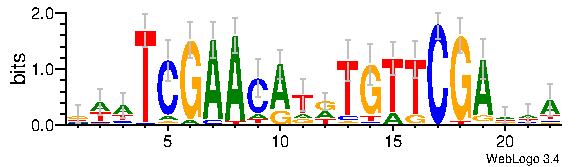
\includegraphics[width=\textwidth]{figures/chapter4/mtuberculosis_motif}
    \caption{\textit{M. tuberculosis}}
  \end{subfigure}
  \begin{subfigure}{0.4\textwidth}
    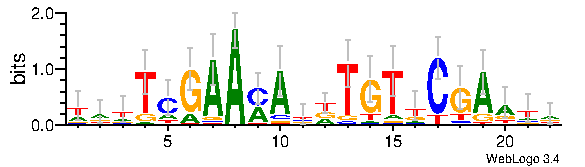
\includegraphics[width=\textwidth]{figures/chapter4/cglutamicum_motif}
    \caption{\textit{C. glutamicum}}
  \end{subfigure}

  \begin{subfigure}{0.4\textwidth}
    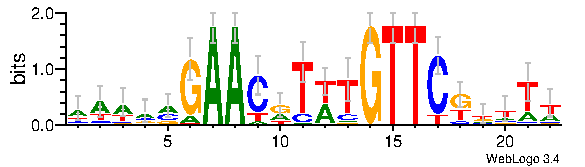
\includegraphics[width=\textwidth]{figures/chapter4/bsubtilis_motif}
    \caption{\textit{B. subtilis}}
  \end{subfigure}
  \begin{subfigure}{0.4\textwidth}
    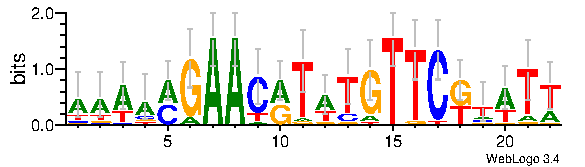
\includegraphics[width=\textwidth]{figures/chapter4/lmonocytogenes_motif}
    \caption{\textit{L. monocytogenes}}
  \end{subfigure}
  \caption{LexA binding motif for the Actinobacteria \textit{M. tuberculosis}
    and \textit{C. glutamicum}, and the Firmicutes \textit{B. subtilis} and
    \textit{L. monocytogenes}.}
  \label{fig:gram-positive-motifs}
\end{figure}

Differences in the LexA-binding motif of Actinobacteria and Firmicutes have
been reported before~\cite{jochmann2009genetic, van2010sos,
  davis2002definition}. It has also been shown that the effect of this
difference on search efficiency can be
significant~\cite{cornish2012inference}. The difference between the
LexA-binding motifs of these two clades (Figure~\ref{fig:gram-positive-motifs})
hence makes the performed analysis an excellent test case to demonstrate the
effectiveness of combining multiple TF binding motifs, with different weights,
to achieve efficient binding site search and regulon inference in all target
genomes.  Figure~\ref{fig:heatmap_1} shows that the binding search efficiency
drops when using the Firmicutes LexA-binding motif on an Actinobacteria genome
and vice versa. As it can be seen, the binding motif of one group does not
detect the two core elements of the SOS response (\textit{lexA} and
\textit{recA} known to be regulated) in all species of the other group.

\begin{figure}
  \centering
  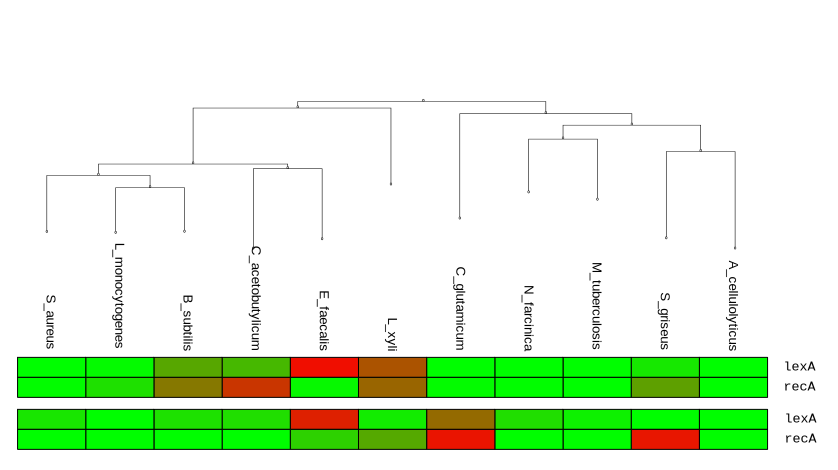
\includegraphics[width=0.7\textwidth]{figures/chapter4/heatmap_single_motif}
  \caption{The heatmaps showing the regulation in groups of orthologous
    \textit{lexA} and \textit{recA} genes. Each row corresponds to an ortholog
    group and organisms (columns) are grouped according to their phylogenetic
    proximity estimated from LexA protein sequences. For each species and
    orthologous group, the posterior probability of regulation is shown in
    green-red shades where green indicates high probability of regulation and
    red denotes low probability. Heatmaps show the results of using
    Actinobacteria (top) and Firmicutes (bottom) LexA-binding motifs to search
    for LexA-binding sites in all species under analysis. The results
    illustrate that clade-specific LexA-binding sites are not generic enough to
    detect binding sites upstream of core SOS response genes \textit{lexA} and
    \textit{recA} in all the species under analysis.}
  \label{fig:heatmap_1}
\end{figure}

In contrast, Figure~\ref{fig:heatmap_2} displays the heatmap of the results
obtained using the motif that is the combination of ones from both Firmicutes
and Actinobacteria.  The core elements of the SOS response, \textit{recA} and
\textit{lexA}, are consistently detected as LexA-regulated in all species. The
maximum likelihood inference of the evolution of \textit{recA} regulation is
shown in Figure~\ref{fig:ASR-a}.  In agreement with the hypothesis that
translesion synthesis (TLS) is a part of core SOS regulon, TLS genes appear to
be regulated by LexA~\cite{erill2007aeons, galhardo2009dinb,
  boshoff2003dnae2}. However, consistent with the experimental data available
for individual organisms, the results show that different genes are involved in
translesion synthesis in each phylum. In the Firmicutes, DNA polymerase IV (encoded
by \textit{dinB}) and UV-damage repair protein UvrX (encoded by \textit{uvrX};
its regulation for ancestral species reconstructed in Figure~\ref{fig:ASR-b})
contribute to the TLS mechanism~\cite{au2005genetic, van2010sos,
  cirz2007complete}. Instead of these two, Actinobacteria utilizes error-prone
DNA-polymerase (encoded by \textit{dnaE2}) as part of the SOS-induced
TLS~\cite{jochmann2009genetic, davis2002definition, boshoff2003dnae2}. In
addition, LexA appears to regulate the expression of \textit{imuA'} which is
involved in DNA damage-inducible mutagenesis and is a component of the
\textit{imuA-imuB-dnaE2}-type mutagenic cassette widespread among bacterial
genomes~\cite{erill2006dispersal}.

\begin{figure}
  \centering
  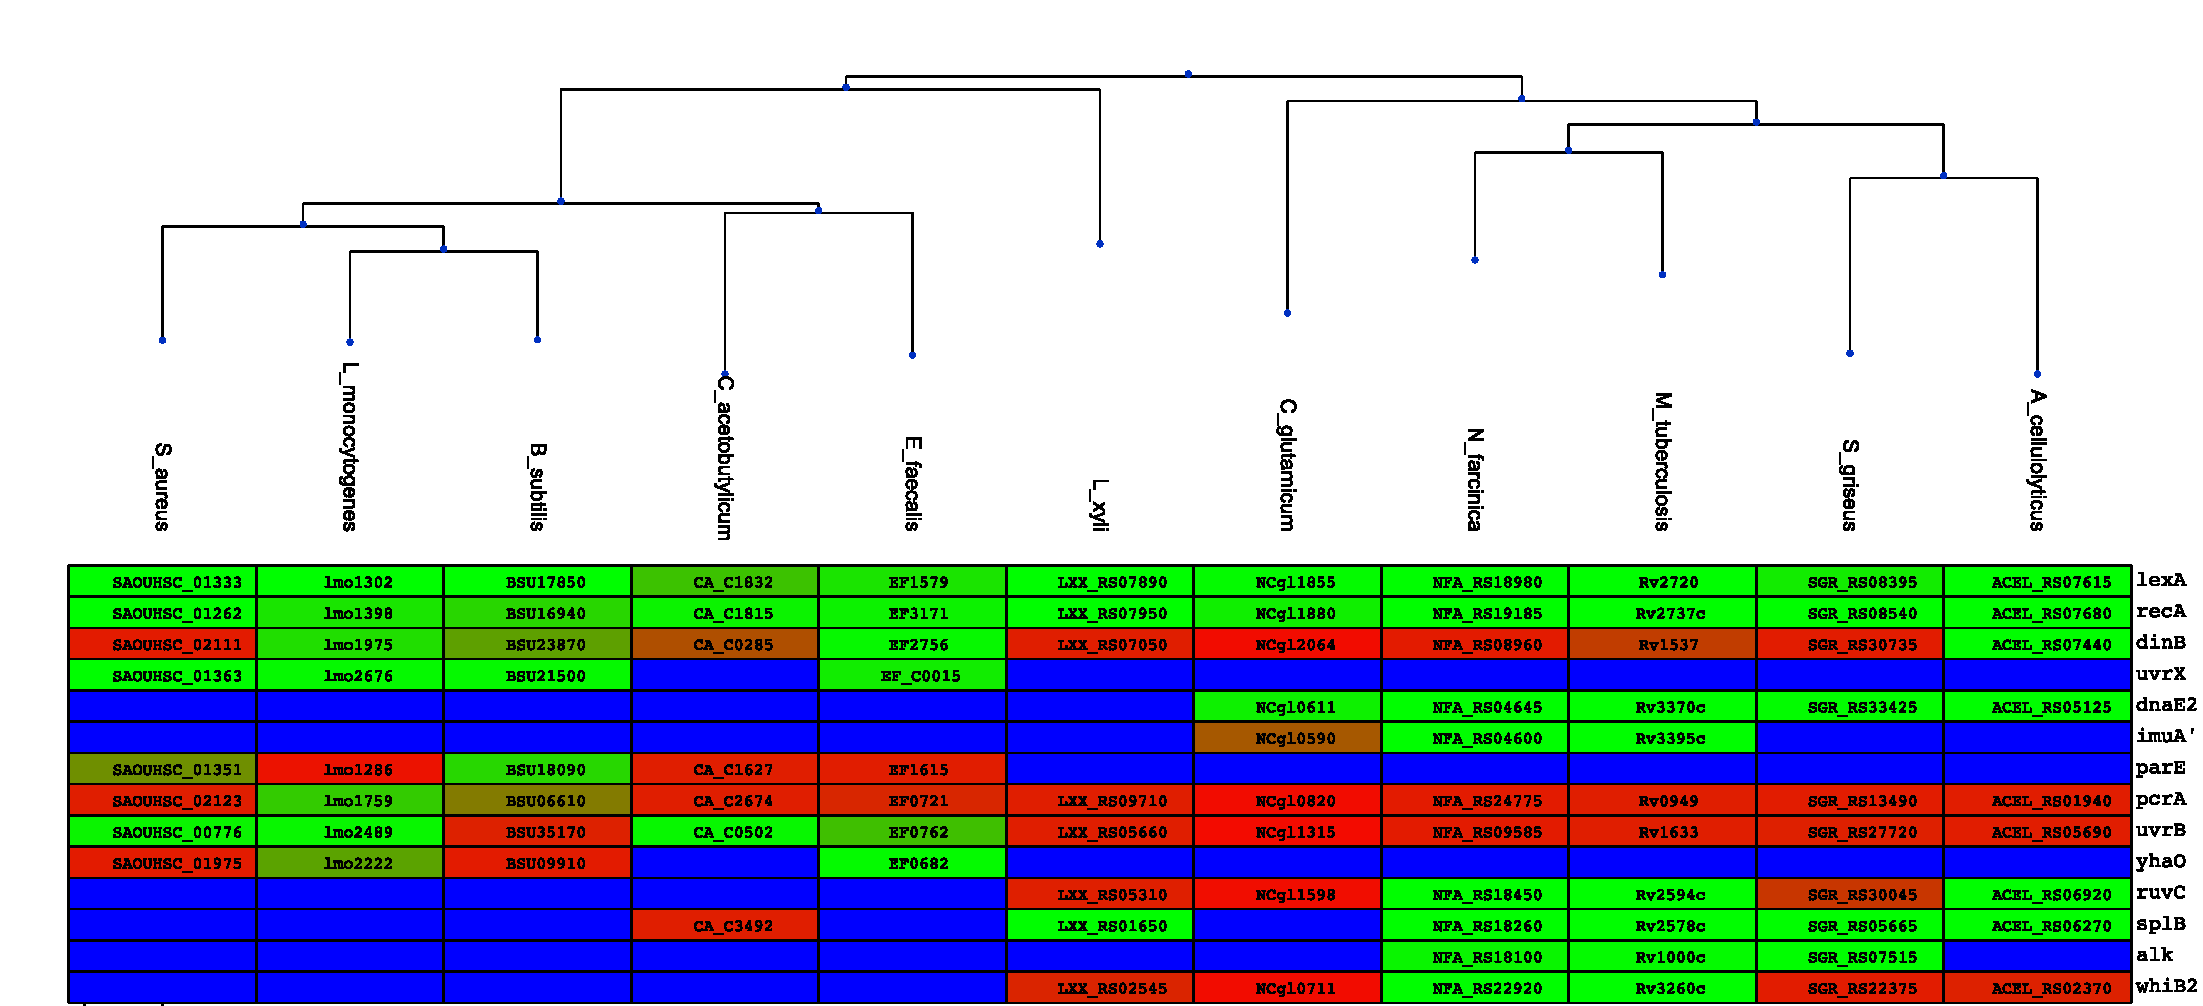
\includegraphics[width=\textwidth]{figures/chapter4/heatmap}
  \caption{The heatmap showing the regulation in selected groups of orthologous
    genes. Each row corresponds to an ortholog group and organisms (columns)
    are grouped according to their phylogenetic proximity estimated from LexA
    protein sequences. For each species and orthologous group, the posterior
    probability of regulation is shown in green-red shades where green
    indicates high probability of regulation and red denotes low
    probability. Blue color indicates that no orthologous gene has been
    identified in a given species for a particular ortholog group. Each cell
    contains the locus tag of its corresponding gene.}
  \label{fig:heatmap_2}
\end{figure}

\begin{figure}
  \centering
  \begin{subfigure}{0.49\textwidth}
    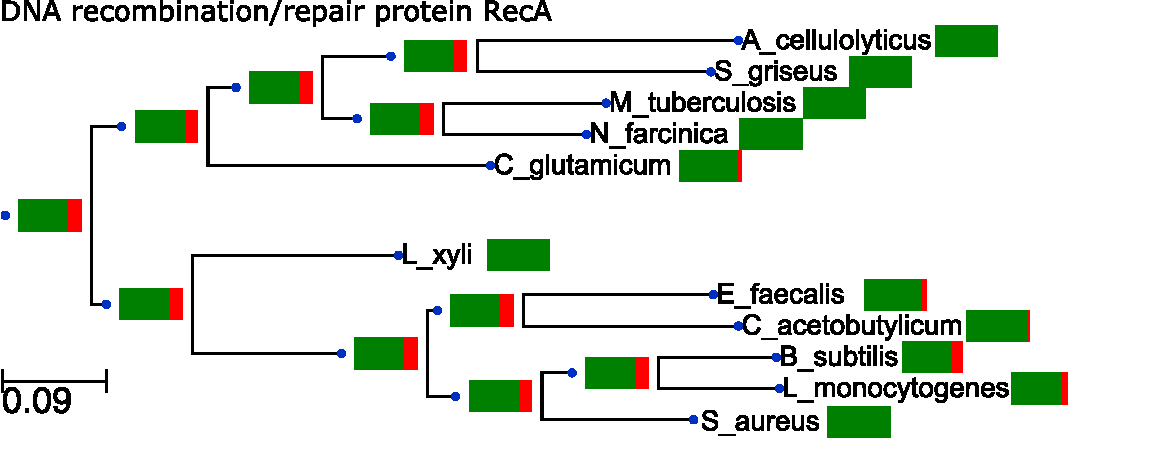
\includegraphics[width=\textwidth]{figures/chapter4/recA_ASR}
    \caption{\textit{recA}}
    \label{fig:ASR-a}
  \end{subfigure}
  \begin{subfigure}{0.49\textwidth}
    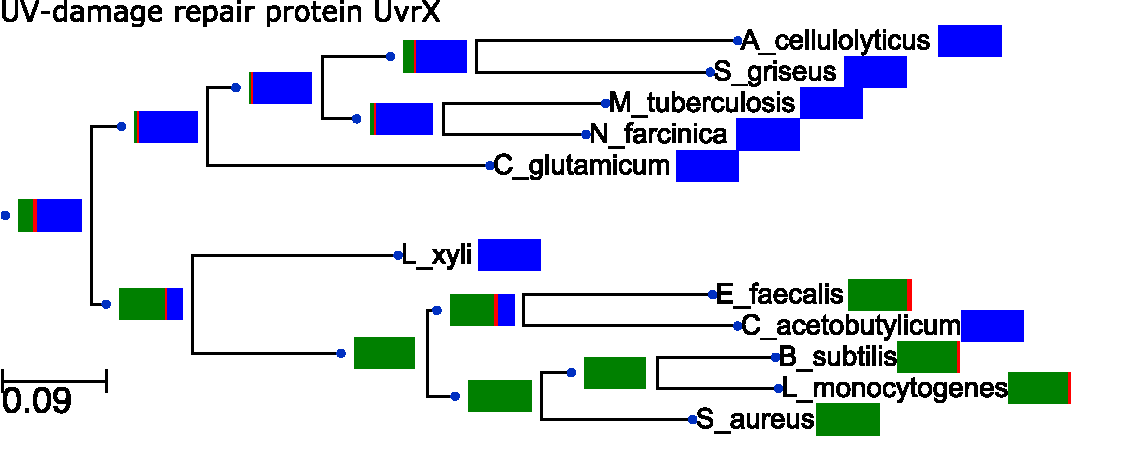
\includegraphics[width=\textwidth]{figures/chapter4/uvrX_ASR}
    \caption{\textit{uvrX}}
    \label{fig:ASR-b}
  \end{subfigure}
  \caption{Ancestral state reconstruction for LexA regulation of DNA
    recombination/repair protein coding \textit{recA} and UV-damage repair
    protein coding \textit{uvrX}. Having high posterior probabilities of
    regulation across all species, \textit{recA} regulation is most likely to
    be present in the most recent common ancestor (MRCA) of Firmicutes and
    Actinobacteria. On the other hand, no \textit{uvrX} ortholog is found in
    the Actinobacteria and in the Firmicutes \textit{C. acetobutylicum}. Absence of
    \textit{uvrX} in species from both phyla suggests that this gene was not present in
    the MRCA of both phyla, but was instead introduced after their split.}
  \label{fig:ASR}
 \end{figure}


 There are several LexA-regulated DNA-repair genes that show a clear
 phylogenetic split between Firmicutes and Actinobacteria. Most Firmicutes
 species maintain SOS regulation of the \textit{uvrBA} operon, yet seem to lack
 the regulation of the Holliday junction resolvase complex (encoded by
 \textit{ruvCAB} operon). In addition, DNA topoisomerase IV subunit B
 (\textit{parE}), ATP-dependent DNA helicase (\textit{pcrA}) and DNA repair
 exonuclease (\textit{yhaO}) appear to be regulated only in Firmicutes. In
 contrast, DNA repair photolyase (\textit{splB}), alkylated DNA repair protein
 (\textit{alk}) and transcriptional regulator WhiB2 (\textit{whiB2}) appear to
 be regulated exclusively in Actinobacteria. These results indicate that the
 composition of the LexA regulon varies significantly across different phyla.





\section{Conclusion}

Despite the ever-growing abundance of experimentally validated TF binding site
data, in a comparative genomics analysis the binding site data for all target
genomes is rarely complete. Therefore, to search for binding sites in species
with no TF-binding evidence and to conduct comparative genomics analysis
including these organisms, it is essential to combine all the available
TF-binding evidence from different species. Existing comparative genomics
platforms for transcriptional regulation analysis lack the methods for
systematic integration of binding evidence from a group of species using
phylogenetic information. In addition, these platforms limit their use to the
species in their system, precluding the characterization of regulatory networks
in species that are either recently sequenced or of special
interest. Furthermore, the lack of a probabilistic framework to integrate
comparative genomics results makes it difficult to assess the confidence in the
predicted binding sites and inferred regulons. Finally, the lack of explicit
use of the phylogenetic relationship between analyzed species makes difficult
to generate and test hypotheses on the evolution of the TF, its binding motifs
and regulons across species.

To address these problems, here we have introduced CGB, a platform for
comparative genomics analysis of bacterial transcriptional regulation. CGB
allows the analysis of any genome that is available in NCBI RefSeq
database. It also combines the binding site collections from multiple sources
and adjusts the contribution of each one based on the phylogenetic distance of
reference and target species. To report putatively regulated operons, it adopts
a Bayesian framework, combining the prior probability of regulation and the
likelihood of a binding site over the entire promoter region into a posterior
probability of regulation which is easier to interpret than raw PSSM
scores. Finally, CGB performs ancestral state reconstruction to infer the
TF-regulation of each gene in all ancestral species which can provide insights
into the evolutionary history of its regulation by the TF\@.

The developed platform was validated with the analysis of LexA regulation in
Gram-positive Bacteria using 11 Firmicutes and Actinobacteria species as target
species and 2 LexA binding motifs from each phylum. The results are consistent
with previous analyses and illustrate how combining binding motifs with the
phylogeny information can adjust for substantial differences in the TF binding
motif. Finally, the analysis shows clear differences in the LexA regulon
composition between Firmicutes and Actinobacteria.


\clearpage
\singlespacing
\bibliographystyle{unsrt}
% github.com/sefakilic/bib
\bibliography{/Users/sefa/Dropbox/bib/bibliography}


\end{document}